% !TeX spellcheck = en_US
\documentclass[11pt, fleqn, titlepage]{article}
%\usepackage{siunitx}
\usepackage{texfiles/SpeedyGonzales}
\usepackage{texfiles/MediocreMike}
\newcommand{\so}[2]{{#1}\mathrm{e}{#2}}
% \geometry{top=1cm}
\usepackage{hyperref}
\hypersetup{
	colorlinks=true,
	linkcolor=blue,
	filecolor=magenta,      
	urlcolor=cyan,
}
\usepackage{subfig}
\usepackage{graphicx}
\title{Human arm trajectories in obstacle avoidance}
\author{Oskar Eiler Wiese Christensen s183917 \\ Anders Henriksen s183904 \\ \\ 02445 Project in Statistical Evaluation of Artificial Evaluation}
\date{\today \vspace{2.5cm} \section*{Abstract} \textit{The summary should contain a summary of the problem that  you are working with, which results you got, as well as main conclusions. \\ Don’t get into technical details. The summary should not be very long} \\ In this paper, the goal is, using the \texttt{armdata.Rdata} dataset, to determine if people can be recognized based on their movements, and if obstacles change the movement curve of the hand of the subject in question.
\\ Lorem ipsum dolor sit amet, consectetur adipiscing elit, sed do eiusmod tempor incididunt ut labore et dolore magna aliqua. Gravida arcu ac tortor dignissim. Et netus et malesuada fames. Convallis posuere morbi leo urna molestie at elementum eu facilisis. Etiam erat velit scelerisque in dictum non. Mollis nunc sed id semper risus in hendrerit gravida. Cursus euismod quis viverra nibh cras pulvinar mattis nunc sed. Eu tincidunt tortor aliquam nulla. Duis convallis convallis tellus id interdum. Nunc lobortis mattis aliquam faucibus purus in massa tempor. Feugiat sed lectus vestibulum mattis ullamcorper. Malesuada proin libero nunc consequat interdum varius. Sed pulvinar proin gravida hendrerit lectus. Varius morbi enim nunc faucibus a. Ultricies leo integer malesuada nunc vel risus commodo viverra maecenas. Id aliquet lectus proin nibh nisl. Ullamcorper velit sed ullamcorper morbi tincidunt.}

\pagestyle{plain}
\fancyhf{}
\rfoot{Page \thepage{} of \pageref{LastPage}}

\graphicspath{{Billeder/}}

\begin{document}

\maketitle
%\thispagestyle{fancy}
%\tableofcontents

\section{Introduction}
\textit{Briefly introduce the background and setting of the problem, as well as the aim of the report. Furthermore, you could give a very short description of the analysis that will be applied.} \\ \\
Security plays a larger role in existence every year, whether used for personal security or for the governmental spying on billions. Throughout the years, sercurity has taken many forms like facial and voice recognition, but movement recognition, if it proves successful, could turn out to be an effective way of finding perpetrators of crimes or locking people into their own homes. For this to truly be effective, it should be possible to classify people based on their movements and maybe even recognize actions based on the motion curve. \\ 
\indent This is exactly what is wished to be accomplished in this paper; Classify the person performing the action based on the given motion curve using decision trees and K-nearest neighbors, and analyzing whether the type of obstacle has an influence on the resulting curve by the use of t-tests and ANOVA. For this, the focus has been specifically on the arm movement dataset from \textbf{Grimme et al. 2014}. The hypothesis prior to the carrying out of the experiment was that it should be possible to classify the person based on the curve, since people can move in substantially different ways. It is also expected that experiment should play a significant role on the resulting curve, since a much taller obstacle should make people lift their arms much more dracstially.

\section{Data}
\textit{Describe of the data you are analyzing. What kinds of data do you have, how were they collected (if applicable)? \\ Include a few good plots to highlight important features in data. You can put additional plots in the appendix.}
\\\\
%*\textbf{Description of data:}
Ten different test subjects performed obstacle avoidance tasks on a table by relocation of a cylindrical object from position A to position B. Different experiments, with varying heights of the obstacle were executed, and the test subjects were furthermore asked to avoid the obstacle by lifting the cylindrical object at hand. The movements were recorded with VZ 4000. The trajectories of markers were recorded using a sampling rate of 110 Hz. The starting position projected to the table is considered the origin in a three dimensional space. Fifteen different obstacle avoidance experiments were conducted, with one experiment for every S,M, or T with the given measure $ d \in \{15, 22.5,  30, 37.5, 45\} $ as well as a control experiment with no obstacle. Each person repeated each of the sixteen different experiments ten times. The full data have a total size of $ m_f = 174,160 $. \cite{armdata}
\begin{figure}[H]
	\centering
	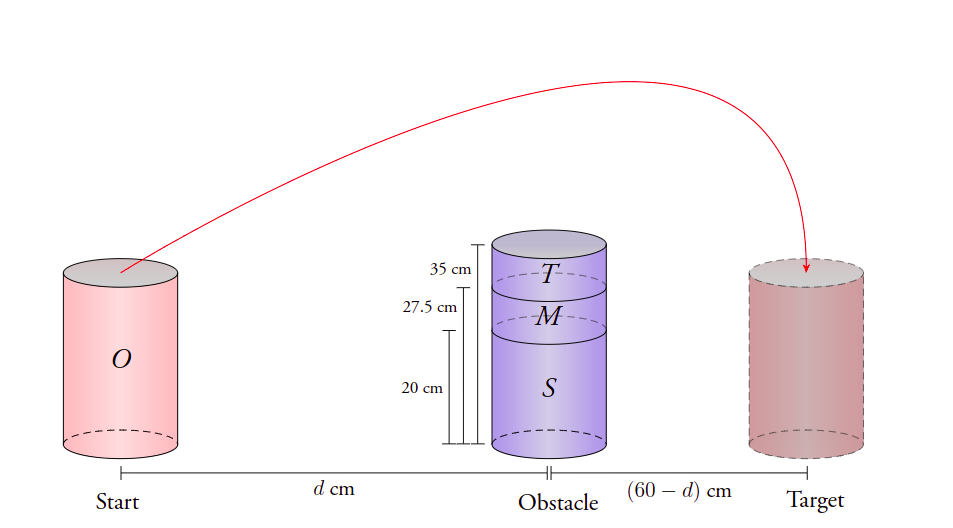
\includegraphics[width=0.7\linewidth]{billeder/exp_pic.png}
	\caption{An illustration of the obstacle avoidance setup. Test subjects have to move the cylinder from start to the finnish position "target", while avoiding the blue obstacle.}
	\label{fig:exppic}
\end{figure}
The data itself consists of recorded trajectory movements, by measured $ x,y,z $-coordinates in a three dimensional space. An illustration of the coordinates are given in \ref{fig:rplot}. Here the variables S, M and T vary in the different experiments. An example of ten different arm-trajectory paths of a test subject repeating the same experiment is shown in the figure \ref{fig:rplot}.

\begin{figure}[H]
	\centering
	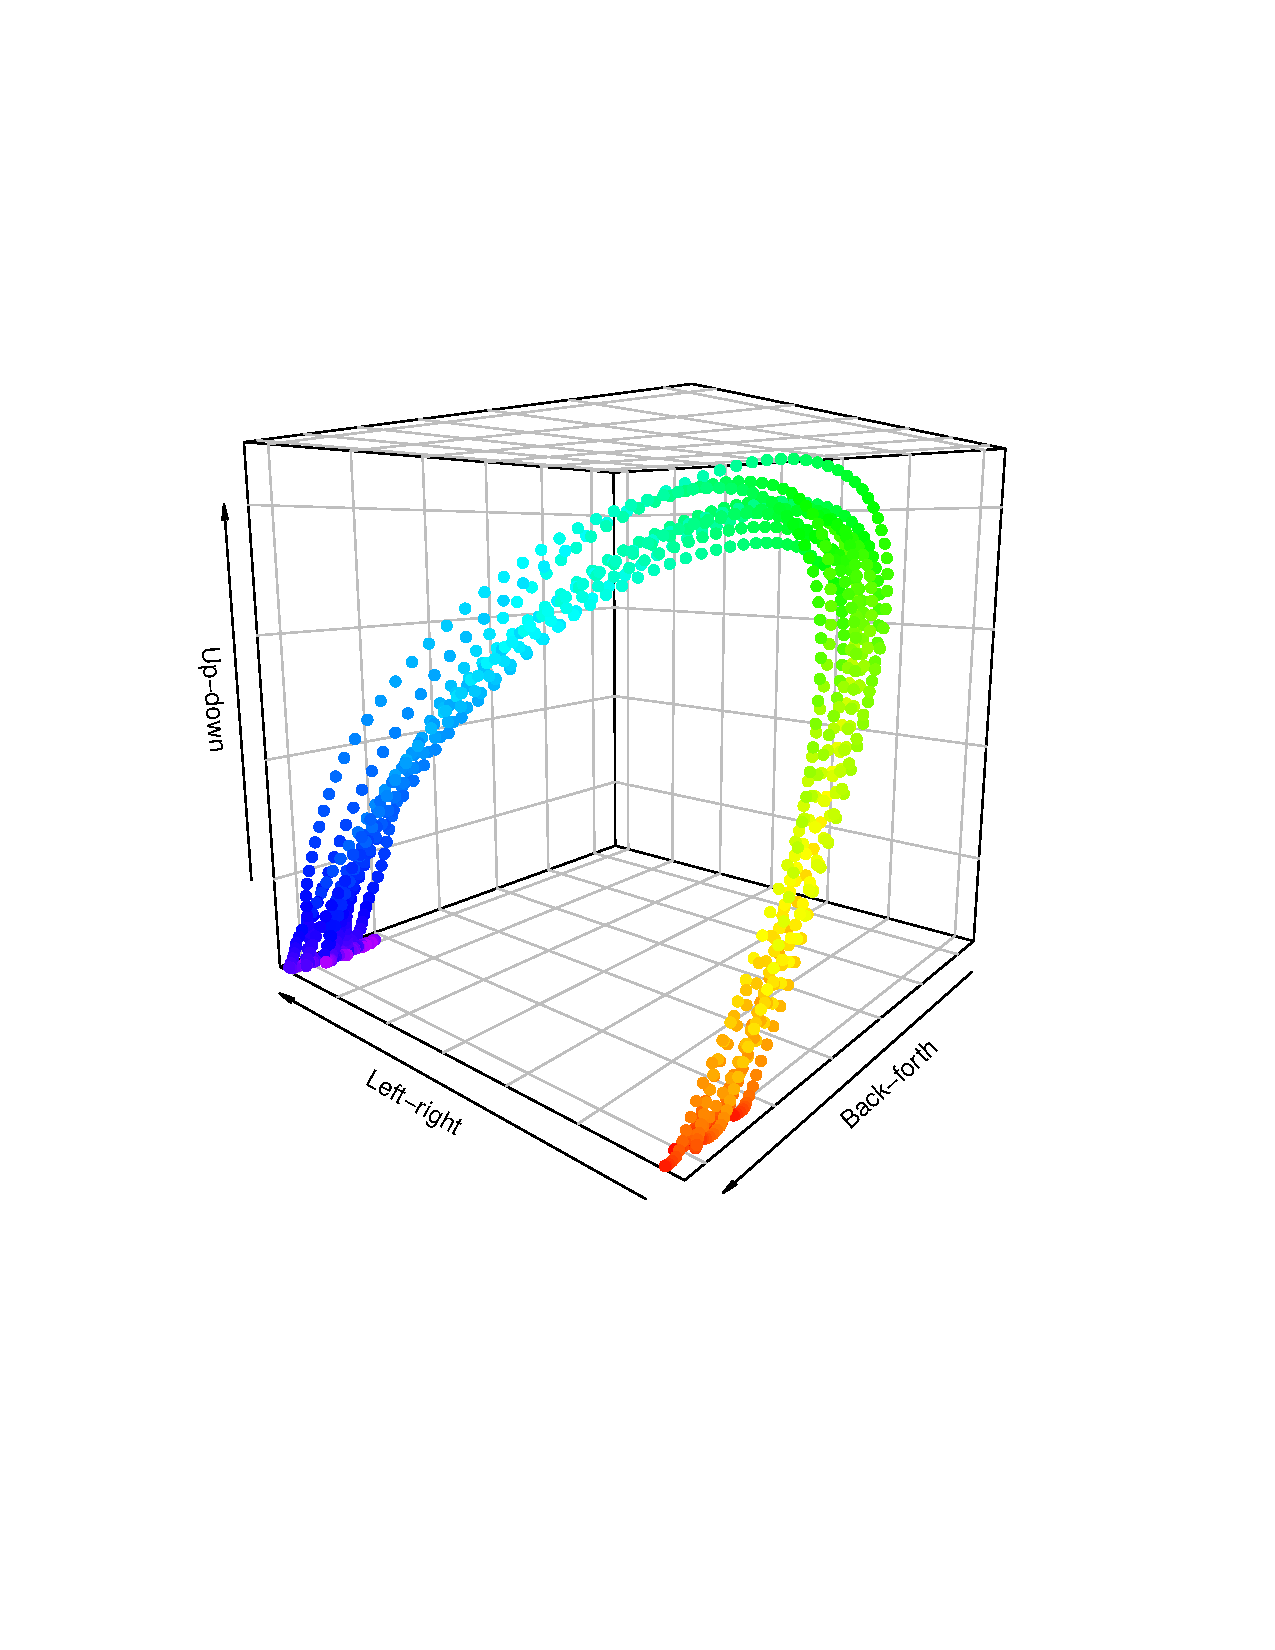
\includegraphics[scale=0.4]{billeder/Rplot.pdf}
	\caption{An illustration of test subject 1's arm trajectories in experiment 1 repetition one through ten}
	\label{fig:rplot}
\end{figure}

%%TODO: forklare lidt om ovenstående. 

\begin{figure}[H]
	\centering
	\includegraphics[width=0.7\linewidth]{billeder/boxplot_z.pdf}
	\caption{Boxplots of the variation in the Z-dimension of the arm trajectories for all test subjects}
	\label{fig:boxplotz}
\end{figure}

Figure \ref{fig:boxplotz} shows a notable variation in the Z-dimension which indicates that it may be possible to distinguish each test subjects trajectory arm movements. In \ref{fig:boxplotz}, the variation is greater for $ z \in [13,85] $ than in the tails, which makes sense since each subject moves the cylindrical object from the same start position to the same end position.
\\\\
A principle component analysis is done in order to investigate the dimensionality and variation of the data. The analysis yields a hundred principle components, whereas a lot of the variation is explained by the first couples as illustrated below, 
\begin{figure}[H]
	\centering
	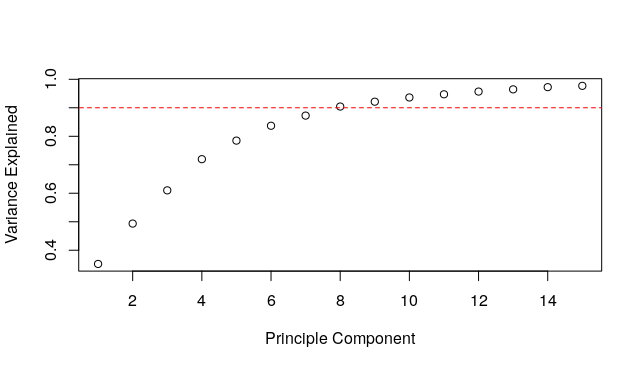
\includegraphics[width=0.7\linewidth]{billeder/varexp.png}
	\caption{}
	\label{fig:varexp}
\end{figure}

In order to explain 90 \% of the variation of the data, the first eight principle components are needed, which also can be noted from figure \ref{fig:varexp}. By having a great proportion of the variance explained by relatively few principle components it seems possible to construct a classifier in order to determine a person from his/her trajectory paths.
\\
To get a visual grasp of the original data points projected onto the space of the principle components, a scatter plot of the transformed data in the principle component space is plotted as seen below,

\begin{figure}[H]
	\centering
	\subfloat[label 1]{{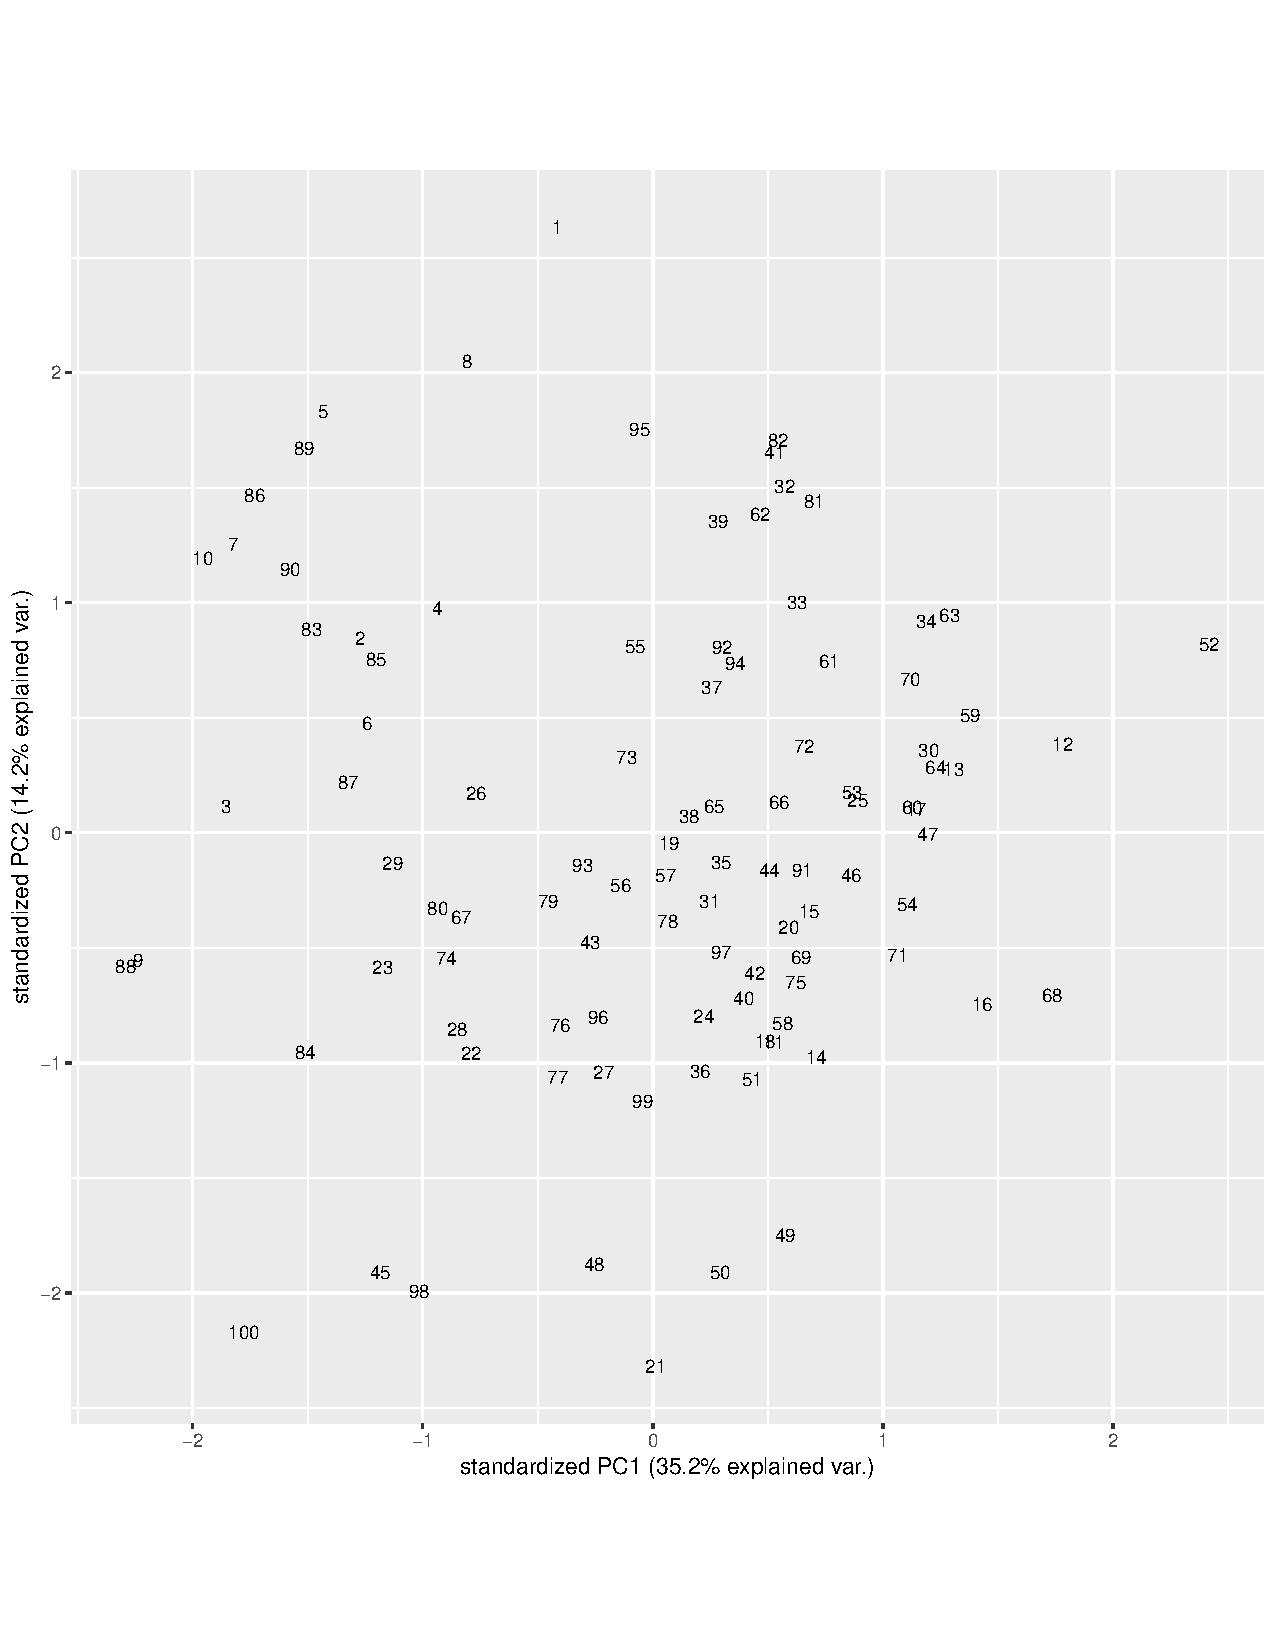
\includegraphics[width=5cm]{billeder/pca1.pdf} }}%
	\qquad
	\subfloat[label 2]{{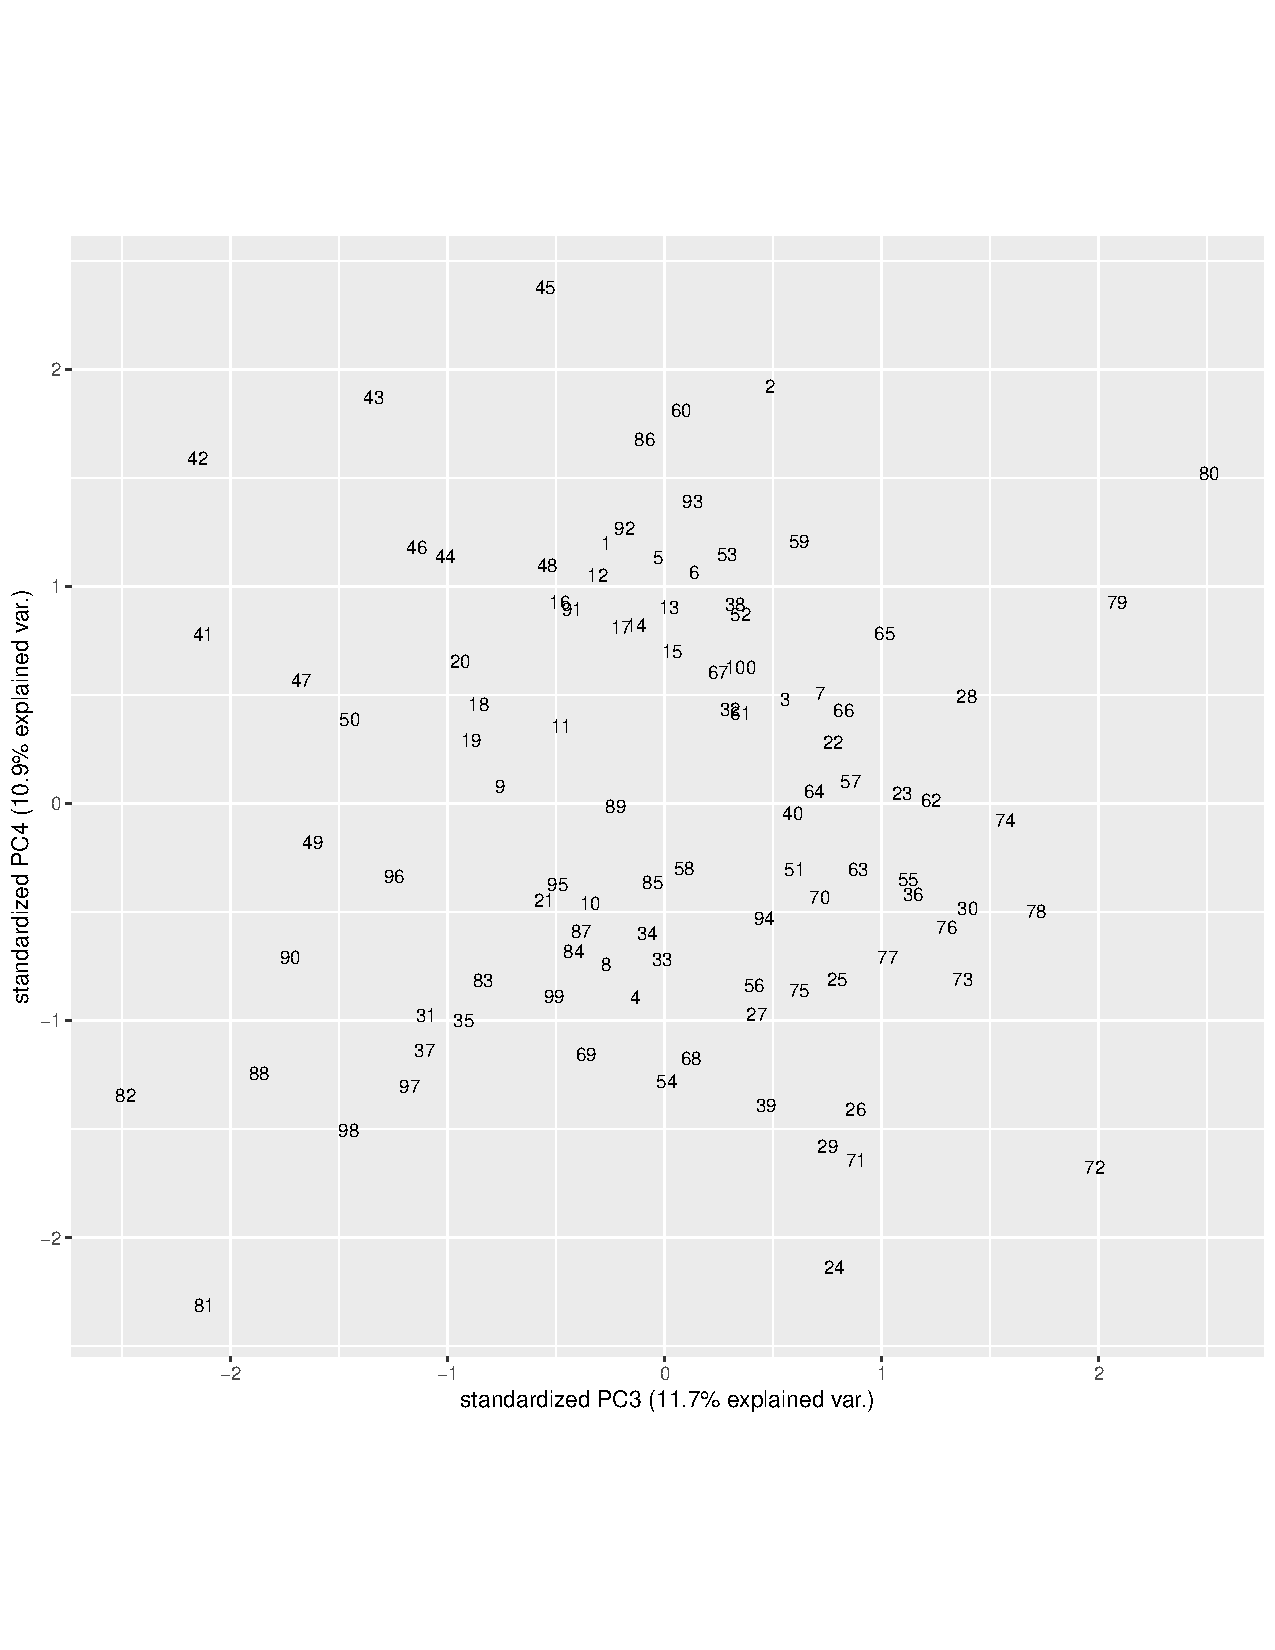
\includegraphics[width=5cm]{billeder/pca2.pdf} }}%
	\caption{Left: A plot of the first two principle components of the data. Right: A plot of the third and fourth principle component. The numbers from 1 to 100 illustrate the date projected onto the principle components}%
	\label{fig:example}%
\end{figure}


\section{Methods}
\textit{Describe the methods you used and why you decided to use them. Also discuss the assumptions behind the methods. Do not go into detail with theory.}

\section{Results}
\textit{Present the results. \\ Tables and figures are good ways of illustrating results.}

\section{Discussion}
\textit{What do your results show? \\ Discuss your results. How reliable are they?}

\section{Conclusion}
\textit{What are your conclusions? The conclusion should be connected to the aim of the report in the introduction. \\ Highlight important results \\ If you have found interesting problems/aspects that you haven’t carried out, you can specify them here as ‘future work’.}

\section{Appendix}


\bibliographystyle{IEEEbib}
\bibliography{refs}

\end{document}
